% Chương 2

\chapter{THUẬT TOÁN TÌM KIẾM} % Tên của chương

\label{Chapter2} % Để trích dẫn chương này ở chỗ nào đó trong bài, hãy sử dụng lệnh \ref{Chapter2} 

%----------------------------------------------------------------------------------------
Thuật toán tìm kiếm theo chiều sâu và chiều rộng là hai thuật toán tìm kiếm mù
phổ biến, thường được sử dụng trong lý thuyết đồ thị. Chúng ta sẽ đi vào từng
thuật toán từ tư tưởng của thuật toán cho tới giả mã và bước đi trong thuật toán để
làm rõ hơn cách thức hoạt động của thuật toán. Trong quá trình tìm hiểu ta sẽ nhận
thấy chúng có nhiều điểm tương đồng trong cách thực hiện, nhưng cách tổ chức thì
khác nhau. Với mỗi thuật toán ta sẽ đưa ra ưu nhược điểm của chúng để có thể sử
dụng chúng phù hợp hơn theo những yêu cầu riêng của bài toán đầu vào.

\section{Thuật toán tìm kiếm theo chiều sâu - Depth First Search (DFS)} 
Trước tiên ta sẽ đi vào tìm hiểu về thuật toán tìm kiếm theo chiều sâu (DFS) \cite{tl2}.
Thuật toán DFS là một quá trình duyệt hay tìm kiếm trên một cây hoặc một đồ thị.
Thuật toán DFS sẽ bắt đầu với một đỉnh gốc và phát triển sâu và xa nhất có thể của
mỗi nhánh. Để hiểu hơn ta sẽ đi vào từng phần trong thuật toán:

\subsection{Tư tưởng của thuật toán}
Với tư tưởng đi sâu vào từng nhánh, ta giả sử đầu vào của thuật toán là một đồ thị
G = (V,E). Coi s là đỉnh gốc của V, ta sẽ bắt đầu quá trình duyệt với s.Từ s ta sẽ đi
thăm tới đỉnh kề với s (giả sử ở đây là u0), từ u0 ta tiếp tục quá trình duyệt với các
đỉnh kề u0 (trừ các đỉnh đã thăm). Quá trình sẽ tiếp tục tới khi gặp đỉnh cần tìm
hoặc đi hết nhánh thì thực hiện lùi lại đỉnh trước đó.

Xét một cách tổng quát thì khi xét một đỉnh u0 ta sẽ có hai khả năng xảy ra:
\begin{itemize}
	\item Nếu như tồn tại đỉnh v0 kề với u0 mà chưa được thăm thì đỉnh v0 đó sẽ được
	đánh dấu để trở thành đỉnh đã thăm và quá trình tìm kiếm sẽ bắt đầu từ đỉnh v0
	đó.
	\item Ngược lại, nếu mọi đỉnh kề với u0 đều đã thăm thì ta sẽ quay lại đỉnh mà trước
	đó ta đến đỉnh u0 để tiếp tục quá trình tìm kiếm
\end{itemize}

Như vậy trong quá trình thăm đỉnh bằng thuật toán tìm kiếm theo chiều sâu, ta
nhận thấy ngay đỉnh càng thăm muộn thì sớm được duyệt trước (đây là cơ chế Last
In First Out) . Do đó ta có thể sử dụng thủ tục đệ quy hoặc sử dụng một danh sách
kiểu ngăn xếp để tổ chức cho quá trình duyệt của thuật toán. Dưới dây là minh họa
cho quá trình duyệt với một cây:

\begin{figure}[h!]
	\centering
	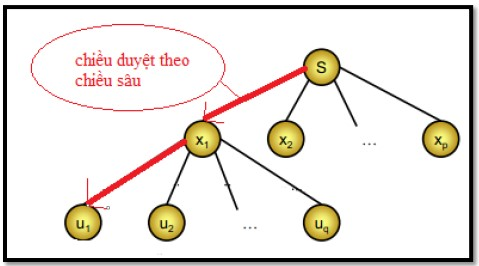
\includegraphics[width=0.8\textwidth]{
		Figures/figs/ThuTuDFS.jpg
	}
	\caption[Thứ tự duyệt của thuật toán DFS]{
		Thứ tự duyệt của thuật toán DFS 
	}
	\label{fig:hinha}
\end{figure}


Hình trên minh họa thứ tự duyệt của thuật toán tìm kiếm theo chiều sâu: ta nhận
thấy từ S sẽ thăm X1, tiếp tục tới u1 là kề với X1. Nếu u1 không phải đỉnh tìm và hết nhánh thì sẽ lùi về X1 để thăm u2. Do đó quá trình duyệt sẽ là: S $\to$ x1 $\to$ u1 $\to$ u2 $\to$ ... $\to$ uq $\to$ x2 $\to$ ...

\subsection{Giải thuật của thuật toán}
Xác định bài toán ta cần lấy ra input và output của bài toán như sau:
\begin{itemize}
	\item \textbf{Input:} đồ thị vào G=(V,E) với đỉnh gốc là s0(Trạng thái đầu)
	
	Tập đích Goal
	\item \textbf{Output:} một đường đi p từ s đến một đỉnh ftrong tập đích Goals
\end{itemize}

Thuật toán DFS có 2 cách để duyệt những đỉnh trong quá trình tìm kiếm đó là sử
dụng thủ tục đệ quy hoặc sử dụng ngăn xếp để lưu trữ các đỉnh sẽ duyệt tiếp đó. Ta
sẽ đi vào cách sử dụng ngăn xếp để lưu trữ các đỉnh.Ta có các bước cho quá trình
thực hiện thuật toán như sau:

\textbf{Bước 1:} khởi tạo
\begin{itemize}
	\item Các đỉnh đều ở trạng thái chưa đánh dấu, trừ đỉnh xuất phát s là đã đánh
	dấu.
	\item Một ngăn xếp S (Stack)ban đầu chỉ đưa vào có một phần tử là s. Bằng việc
	sử dụng ngăn xếp lưu các đỉnh ta sẽ duyệt sâu vào từng nhánh của đồ thị.
\end{itemize}

\textbf{Bước 2:} Lặp lại các bước sau cho đến khi ngăn xếp rỗng:
\begin{itemize}
	\item Nếu ngăn xếp rỗng, không thấy đỉnh đích, thông báo \textit{“không tìm thấy”},
	dừng.
	\item Ngăn xếp không rỗng, lấy u ra khỏi ngăn xếp, thông báo thăm u (bắt đầu
	duyệt đỉnh u, nếu lần đầu thì là u chính là s).
	\item Kiểm tra u có phải đỉnh đích t không:
		\subitem - Nếu đúng trả về u, dừng vòng lặp, chuyển sang bước 3.
		\subitem - Nếu không đúng thì tiếp tục duyệt.
	\item Xét tất cả các đỉnh v kề với u mà chưa được đánh dấu, với mỗi đỉnh v đó:
		\subitem - Đánh dấu v
		\subitem - Ghi nhận đường đi từ v đến u
		\subitem - Đẩy v vào ngăn xếp (v sẽ chờ được duyệt tại những bước sau)
\end{itemize}

\textbf{Bước 3:} Truy ngược lại đường đi (nếu có)

\subsection{Nhận xét}
\begin{itemize}
	\item Có thể có nhiều đường đi từ s $\to$ f, nhưng thuật toán DFS luôn trả về một
	đường đi có thứ tự từ điển nhỏ nhất.
	\item Quá trình tìm kiếm theo chiều sâu cho ta một cây DFS gốc s. Quan hệ chacon trên cây được định nghĩa là: nếu từ đỉnh u tới thăm đỉnh v thì u là nút
	cha của nút v. Hình dưới sẽ minh họa cho cây DFS tương ứng với đỉnh xuất
	phát s=1
\end{itemize}

\begin{figure}[h!]
	\centering
	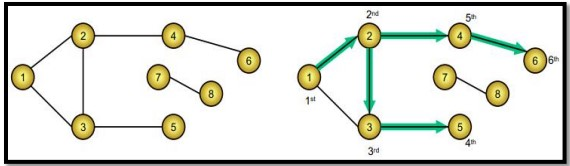
\includegraphics[width=0.8\textwidth]{
		Figures/figs/cayDFS_S1.jpg
	}
	\caption[Cây DFS với s = 1.]{
		Cây DFS với s = 1.
	}
	\label{fig:hinhb}
\end{figure}

\textbf{Ưu điểm}
\begin{itemize}
	\item Nếu bài toán có lời giải, phương pháp tìm kiếm theo chiều sâu đảm bảo tìm
	ra lời giải.
	\item Ký thuật tìm kiếm sâu tập trung vào đích, con người cảm thấy hài lòng khi
	các câu hỏi tập trung vào vấn đề chính.
	\item Do cách tìm của kỹ thuật này, nếu lời giải ở rất sâu, kỹ thuật sâu sẽ tiết
	kiệm thời gian
\end{itemize}

\textbf{Nhược điểm}
\begin{itemize}
	\item Tìm sâu khai thác không gian bài toán để tìm lời giải theo thuật toán đơn
	giản một cách cứng nhắc. Trong quá trình tìm nó không có thông tin nào để
	phát hiện lời giải. Nếu cọn nút ban đầu không thích hợp có thể không dẫn
	tới đích của bài toán.
	\item Không phù hợp với không gian bài toán lớn, kỹ thuật tìm kiếm sâu có thể
	không đi đến lời giải trong khoảng thời gian vừa phải (nếu cố định thời
	gian).
\end{itemize}

%----------------------------------------------------------------------------------------------------------------------------------------------------------------------------------------------------------------------------


\section{Thuật toán tìm kiếm theo chiều rộng (Breadth First Sreach)}
Tương tự thuật toán tìm kiếm DFS thì thuật toán BFS cũng là một thuật toán phổ
biến trong việc tìm kiếm trong đồ thị \cite{tl1}. Nhưng có đôi chút khác biệt về cách tổ chức
các đỉnh để duyệt so với thuật toán DFS. Do đó cách duyệt của BFS cũng trở nên
khác DFS. Để thấy sự khác nhau này ta sẽ đi vào tìm hiểu hơn vào thuật toán.

\subsection{Tư tưởng của thuật toán}
Ta giả sử đầu vào thuật toán là một đồ thị G = (V, E), ta sẽ phải thực hiện lập lịch
duyệt cho các đỉnh của đồ thị G. Việc duyệt các đỉnh sẽ được ưu tiên sao cho đỉnh
nào gần với nó nhất sẽ được duyệt trước. Tức là nó bắt đầu từ mức thấp nhất của
không gian bài toán, sẽ duyệt theo chiều từ trái sang phải hoặc ngược lại ở mức
tiếp theo, nếu không thấy lời giải ở mức này nó sẽ chuyển xuống mức kế để tiếp
tục...cứ như vậy đến khi tìm được lời giải (nếu có). Ta xét ví dụ sau:

Ví dụ : Bắt đầu ta thăm đỉnh S. Việc thăm đỉnh S sẽ phát sinh thứ tự duyệt những
đỉnh (x[1], x[2], .. ,x[p]) kề với S (những đỉnh gần S nhất). Khi thăm đỉnh x[1] sẽ
lại phát sinh yêu cầu duyệt những đỉnh (u[1], u[2], ..., u[q]) kề với x[1]. Nhưng rõ
ràng các đỉnh u này xa S hơn những đỉnh x nên chúng chỉ được duyệt khi tất cả các
đỉnh x đã được duyệt xong. Tức là thứ tự duyệt đỉnh sau khi đã thăm x[1] sẽ là :
(x[2], x[3], ..., x[p], u[1], u[2],..., u[q])

\begin{figure}[h!]
	\centering
	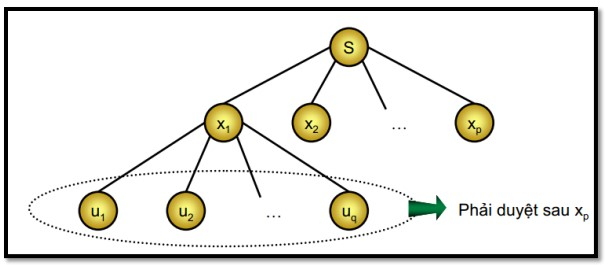
\includegraphics[width=0.8\textwidth]{
		Figures/figs/ThuTuBFS.jpg
	}
	\caption[Thứ tự duyệt thuật toán BFS]{
		Thứ tự duyệt thuật toán BFS
	}
	\label{fig:hinhc}
\end{figure}

\subsection{Giải thuật của thuật toán}
\begin{itemize}
	\item \textbf{Input:} cây đồ thị G= (V,E) với đỉnh gốc là $s_0$ ( trạng thái đầu)
	
	Tập đích Goals.
	\item \textbf{Output:} một đường đi p từ $n_0$ đến 1 đỉnh f trong tập Goals
\end{itemize}

Thuật toán sử dụng một cấu trúc dữ liệu là hàng đợi (Queue) để lưu trữ thông tin
trung gian trong quá trình tìm kiếm (ở đây dễ hiểu là các đỉnh kế tiếp đợi được
duyệt). Tương tự với tìm kiếm theo chiều sâu, các bước cho giải thuật tìm kiếm
theo chiều rộng như sau :

\textbf{Bước 1:} Khởi tạo
\begin{itemize}
	\item Các đỉnh đều ở trạng thái chưa đánh dấu, trừ đỉnh xuất phát s là đã đánh
	dấu.
	\item Một hàng đợi Q (tổ chức dạng hàng đợi Queue), ban đầu chỉ có một phần tử
	là s. Hàng đợi dùng để chứa các đỉnh sẽ được duyệt theo thứ tự ưu tiên
	chiều rộng.
\end{itemize}

\textbf{Bước 2:} Lặp lại các bước sau cho đến khi hàng đợi rỗng
\begin{itemize}
	\item Nếu hàng đợi rỗng, không thấy đỉnh đích, thông báo \textit{“ không tìm thấy”} ,
	dừng.
	\item Hàng đợi không rỗng, lấy u ra khỏi hàng đợi , thông báo thăm u (bắt đầu
	duyệt đỉnh u, nếu là lần duyệt đầu thì u ở đây là s).
	\item Kiếm tra u có phải đỉnh đích t không
		\subitem - Nếu đúng trả về u, dừng vòng lặp, sang bước 3
		\subitem - Nếu sai tiếp tục chương trình.
	\item Xét tất cả các đỉnh v kề với u mà chưa được đánh dấu, với mỗi đỉnh v đó:
		\subitem - Đánh dấu v
		\subitem - Ghi nhận đường đi từ v đến u
		\subitem - Đấy v vào hàng đợi (v sẽ chờ được duyệt tại những bước sau)
\end{itemize}

\textbf{Bước 3:} Truy ngược đường đi

\subsection{Nhận xét}
\begin{itemize}
	\item Có thể có nhiều đường đi từ s tới f nhưng thuật toán BFS luôn trả về một
	đường đi ngắn nhất (theo nghĩa đi qua ít cạnh nhất).
	\item Quá tình tìm kiếm theo chiều rộng cho ta một cây BFS gốc s. Quan hệ cha –
	con trên cây được định nghĩa là : nếu từ đỉnh u tới thăm đỉnh v thì u là nút
	cha của nút v. Hình biểu diễn về cây BFS:
\end{itemize}

\begin{figure}[h!]
	\centering
	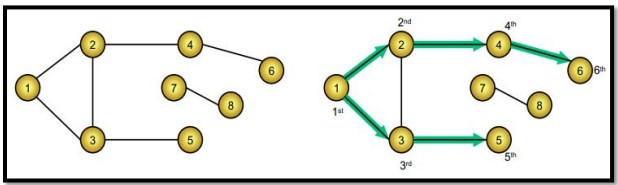
\includegraphics[width=0.8\textwidth]{
		Figures/figs/bieuDienCayBFS.jpg
	}
	\caption[Biểu diễn cây BFS]{
		Biểu diễn cây BFS
	}
	\label{fig:hinhd}
\end{figure}

\textbf{Ưu điểm}
\begin{itemize}
	\item Kỹ thuật tìm kiếm rộng là kỹ thuật vét cạn không gian trạng thái bài toán vì
	vậy sẽ tìm được lời giải nếu có
	\item Đường đi tìm được thỏa mãn đi qua ít đỉnh nhất.
\end{itemize}

\textbf{Nhược điểm}
\begin{itemize}
	\item Tìm kiếm lời giải theo thuật toán đã định trước, do vậy tìm kiếm một cách
	máy móc; khi không có thông tin bổ trợ cho quá trình tìm kiếm, không nhận
	ra ngay lời giải.
	\item Không phù hợp với không gian bài toán có kích thước lớn. Đối với loại bài
	toán này thì phương pháp tìm kiếm chiều rộng đối diện với các khó khăn về
	nhu cầu:
		\subitem - Cần nhiều bộ nhớ theo số nút cần lưu trữ.
		\subitem - Cần nhiều công sức xử lý các nút, nhất là khi các nhánh cây dài, số
		nút tăng.
		\subitem - Dễ thực hiện các thao tác không thích hợp , thừa, đưa đến việc tăng
		đáng kể số nút phải xử lý.
	\item Không hiệu quả nếu lời giải ở sâu. Phương pháp này không phù hợp cho
	trường hợp có nhiều đường dẫn đến kết quả nhưng đều sâu.
	\item Giao tiếp với người dùng không thân thiện. Do duyệt qua tất cả các nút,
	việc tìm kiếm không tập trung vào một chủ đề.
\end{itemize}

\section{Độ phức tạp của BFS và DFS}
Quá trình tìm kiếm trên đồ thị bắt đầu từ một đỉnh có thể thăm tất cả các đỉnh còn
lại, khi đó cách biểu diễn đồ thị có ảnh hưởng lớn tới chi phí về thời gian thực hiện
giải thuật:
\begin{itemize}
	\item Trong các trường hợp ta biểu diễn đồ thị bằng danh sách kề, cả hai thuật
	toán BFS và DFS đều có độ phức tạp tính toán là O(n+m) = O(max(n,m)).
	Đây là cách cài đặt tốt nhất.
	\item Nếu ta biểu diễn đồ thị bằng ma trận kề thì độ phức tạp tính toán trong
	trường hợp này là $O(n+n^2) = O(n^2).$
	\item Nếu ta biểu diễn đồ thị bằng danh sách cạnh, thao tác duyệt những đỉnh kề
	với đỉnh u sẽ dẫn tới việc duyệt toàn bộ danh sách cạnh, đây là cách cài đặt
	tồi tệ nhất, nó có độ phức tạp tính toán là O(n.m).
\end{itemize}





